\subsection{The Max-Max Similarity Function}
%We now give a general framework of measuring the semantic similarity between
%terms using the concept clustering. As shown in Algorithm \ref{alg:refined},
%our clustering-based approach also has three steps similar to the basic approach.
%% That is, we first judge the type of terms. Second, we represent the semantic contexts of each term according to its type, that is, modeling a probability distribution over contexts. Third, we compare how similar these two discrete probability distributions are by encoding them as vectors and computing the cosine between the vectors.
%The difference is that we add the clustering in Algorithm \ref{alg:conceptClustering}
%on all concept contexts of terms for their possible senses,
%and then evaluate the semantic similarity by comparing these
%concept-cluster contexts. We will give the details on the
%concept-cluster-based similarity evaluation in the following section.
%
%
%\subsubsection{Context Comparison}
In the basic approach, we compute the similarity of two terms by the
cosine similarity between their contexts (\eqnref{eq:cosine}).
In the refined approach, we use a new similarity function known as
{\em max-max similarity}.
%We formalize the concept cluster-based context comparison method as follows.
Let $C=\{C_1,C_2,...,C_k\}$ be clusters of all concepts in $\Gamma_{isA}$,
$C^{t_1}$ and $C^{t_2}$ be the sets of concepts that two terms belong to
respectively. According to the cluster information in $C$,
we divide $C^{t_1}$ and $C^{t_2}$ into small clusters
$C^{t_1}=\{C^{t_1}_{1},..., C^{t_1}_{m}\}$ and
$C^{t_2}=\{C^{t_2}_{1},..., C^{t_2}_{n}\}$ by
comparing $C^{t_1} \cap C$ and $C^{t_2} \cap C$ respectively.
We then compute the similarity between the contexts of each cluster pair
and get the semantic similarity between two terms as:
\begin{equation}
\begin{aligned}
sim(T(t_{1}), T(t_{2})) = \max_{x, y}\{cosine(C^{t_1}_{x}, C^{t_2}_{y})\}
\label{eq:clusterCosine}
\end{aligned}
\end{equation}
where $1\leq x \leq m$ and $1 \leq y \leq n$.

With all concepts clustered offline and the new similarity function
based on concept clusters, the refined algorithm is given in
Algorithm \ref{alg:refined}.
%
% \begin{table}[!h]
% \centering
% \caption{Concept clusters of a pairwise term Microsoft and Apple}% (extracted using Hearst patterns)}
% \label{tab:microsoft-apple-clusters}
% \begin{tabular}{|p{2pt}|l|c|p{2pt}|l|c|}\hline
%  & concepts &  &  & concepts & \\
% id & of Microsoft & weight & id & of Apple & weight\\\hline
% 1	&company	&0.3738	&1	&fruit	&0.2952\\
% 1	&u.s. company	&0.0349	&1	&seasonal fruit	&0.0826\\
% 1	&client	&0.0256	&1	&tree fruit	&0.0048\\
% 1	&large company	&0.0227	&1	&fresh fruit	&0.0389\\
% 1	&software giant	&0.0217	&1	&juice	&0.0067\\
% 	&international-&	&	&	&\\
% 1	&company	&0.0207	&1	&fruit juice	&0.0065\\
% 	&technology-	&	&	&	&\\
% 1	&company	&0.0145	&1	&dried fruit	&0.0051\\
% 1	&software company	&0.0141	&2	&company	&0.1239\\
% 1	&big company	&0.0125	&2	&manufacturer	&0.0100\\
% 1	&giant	&0.0123	&2	&competitor	&0.0077\\
% 1	&player	&0.0112	&2	&large company	&0.0048\\
% 1	&software vendor	&0.0095	&3	&food	&0.0612\\
% 1	&competitor	&0.0086	&3	&snack	&0.0054\\
% 1	&partner	&0.0082	&3	&healthy snack	&0.0052\\
% 1	&manufacturer	&0.0071	&4	&fruit tree	&0.0223\\
% 1	&industry giant	&0.0068	&4	&tree	&0.0083\\
% 1	&big player	&0.0063	&5	&brand	&0.0216\\
% 2	&organization	&0.0217	&6	&crop	&0.0147\\
% 3	&provider	&0.0184	&7	&flavor	&0.0121\\
% 4	&industry leader	&0.0184	&8	&product	&0.0067\\
% \hline
% \end{tabular}
% \end{table}
%
%For example, Table~\ref{tab:microsoft-apple-clusters} shows the top 20 concepts of the entity pair $<microsoft,~apple>$, according to the cluster information in $C$, we can get the clusters that each concept belongs to. In terms of Eq.~\ref{eq:clusterCosine}, we can get the maximum similarity score of this pair, namely the cosine score by comparing the context of Microsoft in the $1^{st}$ cluster with that of Apple in the $2^{nd}$ cluster. In this case, the similarity score between Microsoft and Apple is improved from 0.378 in Eq.~\ref{eq:cosine} to 0.994 in Eq.~\ref{eq:clusterCosine}.
%
%\makeatletter\def\@captype{algorithm}\makeatother
%\KZ{Is it possible to simplify this algo? The structure looks the same as
%Algo 1.} \LP{revised}

\renewcommand\algorithmicrequire{\textbf{Input:}}
\renewcommand\algorithmicensure {\textbf{Output:}}
\begin{algorithm}[th]
%\begin{center}
\caption{Refined Approach}
\label{alg:refined}
\begin{algorithmic}[1]
\REQUIRE \pair{t_1}{t_2}: a pair of terms;\\
~~~~~~$\Gamma_{isA}$: the semantic network of isA relationship;\\
~~~~~~$\Gamma_{ssyn}$: the synset data set in $\Gamma_{isA}$;\\
~~~~~~$\Gamma_{cluster}$: clusters of all concepts in $\Gamma_{isA}$;
\ENSURE a similarity score of \pair{t_1}{t_2};
\STATE Install the synset checking and type checking as Steps 1-4 in Algorithm \ref{alg:baseline};
\IF {\pair{t_1}{t_2} is a concept pair}
\STATE return $sim(\mathcal{I}_c^{t_1}, \mathcal{I}_c^{t_2})$ as Steps 6-7 in Algorithm \ref{alg:baseline};
\ENDIF
\IF {\pair{t_1}{t_2} is an entity pair}
\STATE $sim_1\leftarrow sim(\mathcal{I}_e^{t_1}, \mathcal{I}_e^{t_2})$ as Steps 10-11 in Algorithm \ref{alg:baseline};
\STATE Find clusters of contexts $C^{t_1}$ and $C^{t_2}$ from $\Gamma_{cluster}$;% and prune the cluster sets;
\STATE $sim_2\leftarrow sim(C^{t_1}, C^{t_2})$ computed in \eqnref{eq:clusterCosine};
\STATE return $max(sim_1, sim_2)$;
\ENDIF
\IF {\pair{t_1}{t_2} is a concept-entity pair}
\STATE Collect all concepts of the entity term $t_i$ from $\Gamma_{isA}$ as the context $C^{t_i} (i\in\{1, 2\})$;
\STATE Find clusters of contexts $C^{t_i}$ from $\Gamma_{cluster}$;% and prune the cluster sets;
\FOR {each cluster $C_x$ in $C^{t_i}$}
\STATE Select top $K$ concepts to represent $t_i$, namely $C{^{K}_{x}}=\{c_y|c_y \neq t_j,c_y\in C_x, 1\leq y \leq K\}$;
\FOR {each concept $c_y$ in $C{^{K}_{x}}$}
\STATE $sim_{c_y}\leftarrow$ get the semantic similarity between $c_y$ and $t_j$ by repeating this algorithm iteratively;
\ENDFOR
\STATE $sim_{C_x}\leftarrow max_{c_y\in C{^{K}_{x}}}\{sim_{c_y}\}$;
\ENDFOR
\STATE return $max\{sim_{C_x}|C_x\in C^{t_i}\}$;
\ENDIF
\end{algorithmic}
%\end{center}
\end{algorithm}


\subsection{Optimization by Cluster Pruning}
%We now discuss the advantage and disadvantage using the clustering-based approach for measuring semantic similarity between terms.
%Table~\ref{tab:examples} compares the semantic similarity scores of 9 pairs predicted in Eq.~\ref{eq:clusterCosine} and Eq.~\ref{eq:cosine}. From the experimental results, we can see that comparing the baseline approach using Eq.~\ref{eq:cosine}, our clustering-based approach using Eq.~\ref{eq:clusterCosine} ac
%tually improve the semantic similarity of pairs, such as $<Apple,~Microsoft>$, $<Orange,~Red>$ and $<Microsoft, GE>$ those with ambiguous terms whose data d
%istributions of senses hidden in contexts are skewed. However, it also improves the similarity score of dissimilar pairs like $<lunch,~music>$. This is cause by the following reasons.
The cluster-based refined approach improves the quality of similarity remarkably from
the basic algorithm. But there are two problems. First, the max-max similarity function tends to boost the probability of picking
a less dominant sense of a term because it is easier for 
small clusters to look similar
by the cosine similarity and hence dominate the max-max similarity score. However, many small clusters in $C$ are usually noises. This leads to incorrect
similarity results.
%
%First, there are some noisy concepts in the tail of the concept context given a term, which lead to many small sized clusters formed when using the offline
%clustering method.
%For example, as shown in Table~\ref{tab:microsoft-apple-clusters}, there are small clusters like crop and flavor in the top 20 concepts of Apple, which does
% not accurately represent a sense of Apple.
Second, with the current concept clustering algorithm, some terms can have both
a general sense and a more specific sense. For example, the term ``lunch'' has a specific
sense called ``dish'' and a more general (and also vague) sense called ``activity''.
We know ``activity'' is  more general because it is a superconcept of ``disk''
in $\Gamma_{isA}$. Such general senses poses problems because they make almost
unrelated terms similar. For example, the term ``music'' also has the ``activity'' sense
and thus is deemed similar to ``lunch''.
%
%some term we can get some general (vague) senses except of specific senses when clustering the concept context, because we clustering all concepts flatly. For
% example, considering the senses of Music and Lunch as shown in Table~\ref{tab:sensesOfSamples}, we call the Activity sense as a vague sense and the dish and multimedia senses as specific ones. This is because the former is a super concept of the latter according to the isA relationships in $\Gamma_{isA}$, whose importance as the sense of the term is less than the latter.
%

To overcome these problems, we adopt an optimization technique called
{\em cluster pruning} after concept clustering.
First, to reduce the negative impact from noisy clusters,
we prune away those clusters with only one member or with very small combined weight.
% the weight is lower than the threshold $\tau$ (e.g., 0.01).
%We use the normalized sum typicality of scores for the term \emph{e}
%and its concept $c_i$ in a cluster $C_x$ as the weight of the current cluster.
The weights of clusters are computed below. Let the concept clusters of the term \emph{t} be $C^t = \{C^t_1,...,C^t_m\}$,
the weight of each cluster $C_x^{t}$ is $w_x/\sum_{x}w_x$, where
$w_x = \sum_{c_i\in C_x^{t}}p(c_i|t)$ and $1 \leq x \leq m$.
%In this processing, we can get more accurate senses for each terms. For example, Table~\ref{tab:sensesOfSamples} summarizes main senses of ambiguous terms in Table~\ref{tab:examples} according to the cluster centers and their weights.
Second, to avoid the impact from the vague senses, we prune the clusters
whose senses are superconcepts of other senses according to the isA relationships
in $\Gamma_{isA}$. For example, Fig.~\ref{fig:clusters-given-a-pair}
shows a hierarchical isA relationships of senses after clustering concept
contexts of two terms ``lunch'' and ``music''. Because the senses ``Activity'',
``Cost'', ``Interest'' and ``Art'' are the superconcepts of the senses ``Dish'' and
``Multimedia'', we only keep specific senses like ``Dish'' and ``Multimedia'' and
remove the rest.
%then we compare their contexts in the clusters in Eq.~\ref{eq:clusterCosine}.
%Finally, we can get the similarity between Lunch and Music,
%which is reduced to \textbf{0.012}.

%\begin{table}[!t]
%\centering
%\caption{Main senses of sampling terms}
%\label{tab:sensesOfSamples}
%\begin{tabular}{|c|c|c|c|} \hline
%entity &id &	senses	&weight\\\hline
%	&1	&Fruit & 0.792\\
%Apple	&2	&Company &0.138\\
%	&3	&Fruit Tree & 0.080\\\hline
%	&1	&Fruit & 0.457\\
%Orange	&2	&Color &0.447\\
%	&3	&Company&0.014\\\hline
%GE	&1	&Company & 0.606\\
%	& 2	&Material&0.394\\\hline
%	&1	&Interest &0.518\\
%Music	&2	&Multimedia&0.201\\
%	&3	&Activity & 0.196\\
%	&4	&Art&0.085\\\hline
%	&1	&Dish &0.501\\
%Music	&2	&Activity&0.251\\
%	&3	&Cost&0.248\\\hline
%Pear	&1	&Fruit & 0.824\\
%	&2	&Fruit Tree & 0.097\\\hline
%Microsoft	&1	&Company &0.895\\\hline
%\end{tabular}
%\end{table}

\begin{figure}[th]
 \centerline{
 \includegraphics[width=0.9\columnwidth]{clusters-given-a-pair.eps}}
\caption{Illustration to vague and specific senses of terms lunch and music} \label{fig:clusters-given-a-pair}
\end{figure}


